%%%%%%%%%%%%%%%%%%%%%%%%%%%%%%%%%%%%%%%%%%%%%%%%%%%%
\graphicspath{{}{appendices/figs/}{appendices/}}
\subsection{Kinematical Distributions at DUNE ND}
%
\label{subsec:kine}

In this section we explore the trident signal in more detail, showing some relevant kinematical distributions for coherent and diffractive events. For concreteness, and due to its large number of events, we choose to focus on the DUNE ND, only commenting slightly on the signal at the lower energies of SBN and $\nu$STORM. The observables we calculate are the invariant mass of the charged leptons $m^2_{\ell^+ \ell^-}$, their separation angle $\Delta \theta$ and their individual energies $E_\pm$. The flux convolved distributions of these observables are shown for the DUNE ND in neutrino mode in \reffig{fig:DUNE_ND_dist}. In these plots, we sum all trident channels with a given undistinguishable final-state proportionally to their rates, although $\nu_\mu$ initiated processes always dominate. The coherent and diffractive contributions are shown separately and on the same axes, but we do not worry about their relative normalization. Other potentially interesting quantities are the angle between the cone formed by the two charged leptons and the beam, $\alpha_C$, and the angle of each charged lepton with respect to the beam direction, $\theta_\pm$.  These additional observables are explored in \refapp{app:distributions}. We also report the distributions of the momentum transfer to the hadronic system, $Q^2$. Although this is not a directly measurable quantity, it is a strong discriminant between the coherent and diffractive processes. We do not present the antineutrino distributions here, but they are qualitatively similar.

Perhaps one of the most valuable tools for background suppression in the measurement of the $\mu^+\mu^-$ trident signal at CHARM~II, CCFR and NuTeV \cite{Geiregat:1990gz,Mishra:1991bv,Adams:1998yf} was the smallness of the invariant mass $m^2_{\ell^+ \ell^-}$. This feature, shown here on the top row of \reffig{fig:DUNE_ND_dist}, is also present at lower energies, where the distributions become even more peaked at lower values; although, the diffractive events tend to be have a more uniform distribution in this variable. This is also true for the angular separation $\Delta \theta$, where coherent dimuon tridents tends to be quite collimated, with $90\%$ of events having $\Delta \theta < 20^\circ$, whilst diffractive ones are less so, with only $47\%$ of events surviving the cut. This difference is much less pronounced for mixed and dielectron channels, where only half of our coherent events obey $\Delta \theta < 20^\circ$, when $37\%$ of diffractive events do so.

An interesting feature of same flavour tridents induced by a neutrino (antineutrino) is that the negative (positive) charged lepton tends to be slightly more energetic than its counterpart, whilst for mixed tridents muons tend to carry away most of the energy. These considerations are also reflected in the angular distributions. The most energetic particle is also the more forward one. For instance, in mixed neutrino induced tridents, $\sim 80 \%$ of the $\mu^-$ are expected to be within $10^\circ$ of the beam direction, whilst only $\sim 35 \%$ of their $e^+$ counterparts do so (see \refapp{app:distributions} for additional distributions).

Finally, we mention that detection thresholds can also be important for trident channels with electrons in the final-state. Assuming, for example, a detection threshold for muons and electromagnetic (EM) showers of 30 MeV in LAr, we end up with efficiencies of (99\%, 71\%, 77\%, 86\%) for ($\mu^+ \mu^-$, $e^+ e^-$, $e^+ \mu^-$, $e^- \mu^+$) coherent tridents. These efficiencies become (96\%, 91\%, 93\%, 96\%) for diffractive tridents, dropping for $\mu^+\mu^-$ and increasing for all others. For comparison, at the lower neutrino energies of SBND and assuming the same detection thresholds, the efficiencies for coherent and diffractive tridents are slightly lower, (97\%, 57\%, 67\%, 77\%) and (90\%, 81\%, 85\%, 90\%) respectively.

While trident events are generally quite forward going, their angular behaviour is quite interesting. We consider here the angle between the charged lepton cone and the neutrino beam, $\alpha_C$, defined as 
%
\[
\cos{\alpha_C} = \frac{ (\vec{p}_3 + \vec{p}_4)  \vdot \vec{p}_1}{ |\vec{p}_3 + \vec{p}_4| |\vec{p}_1| }\, ,\]  
%
and in the individual angle of the charged lepton to the neutrino beam, $\theta$. For same flavour tridents we define $\theta$ for each charge of the visible final-state, whilst for mixed tridents we use their flavour. We also show the distribution in $Q^2 = {-q^2}$, where $q = (P - P^\prime)$, which is of particular interest when considering coherency and the impact of form factors.

\begin{figure}[H]
\centering
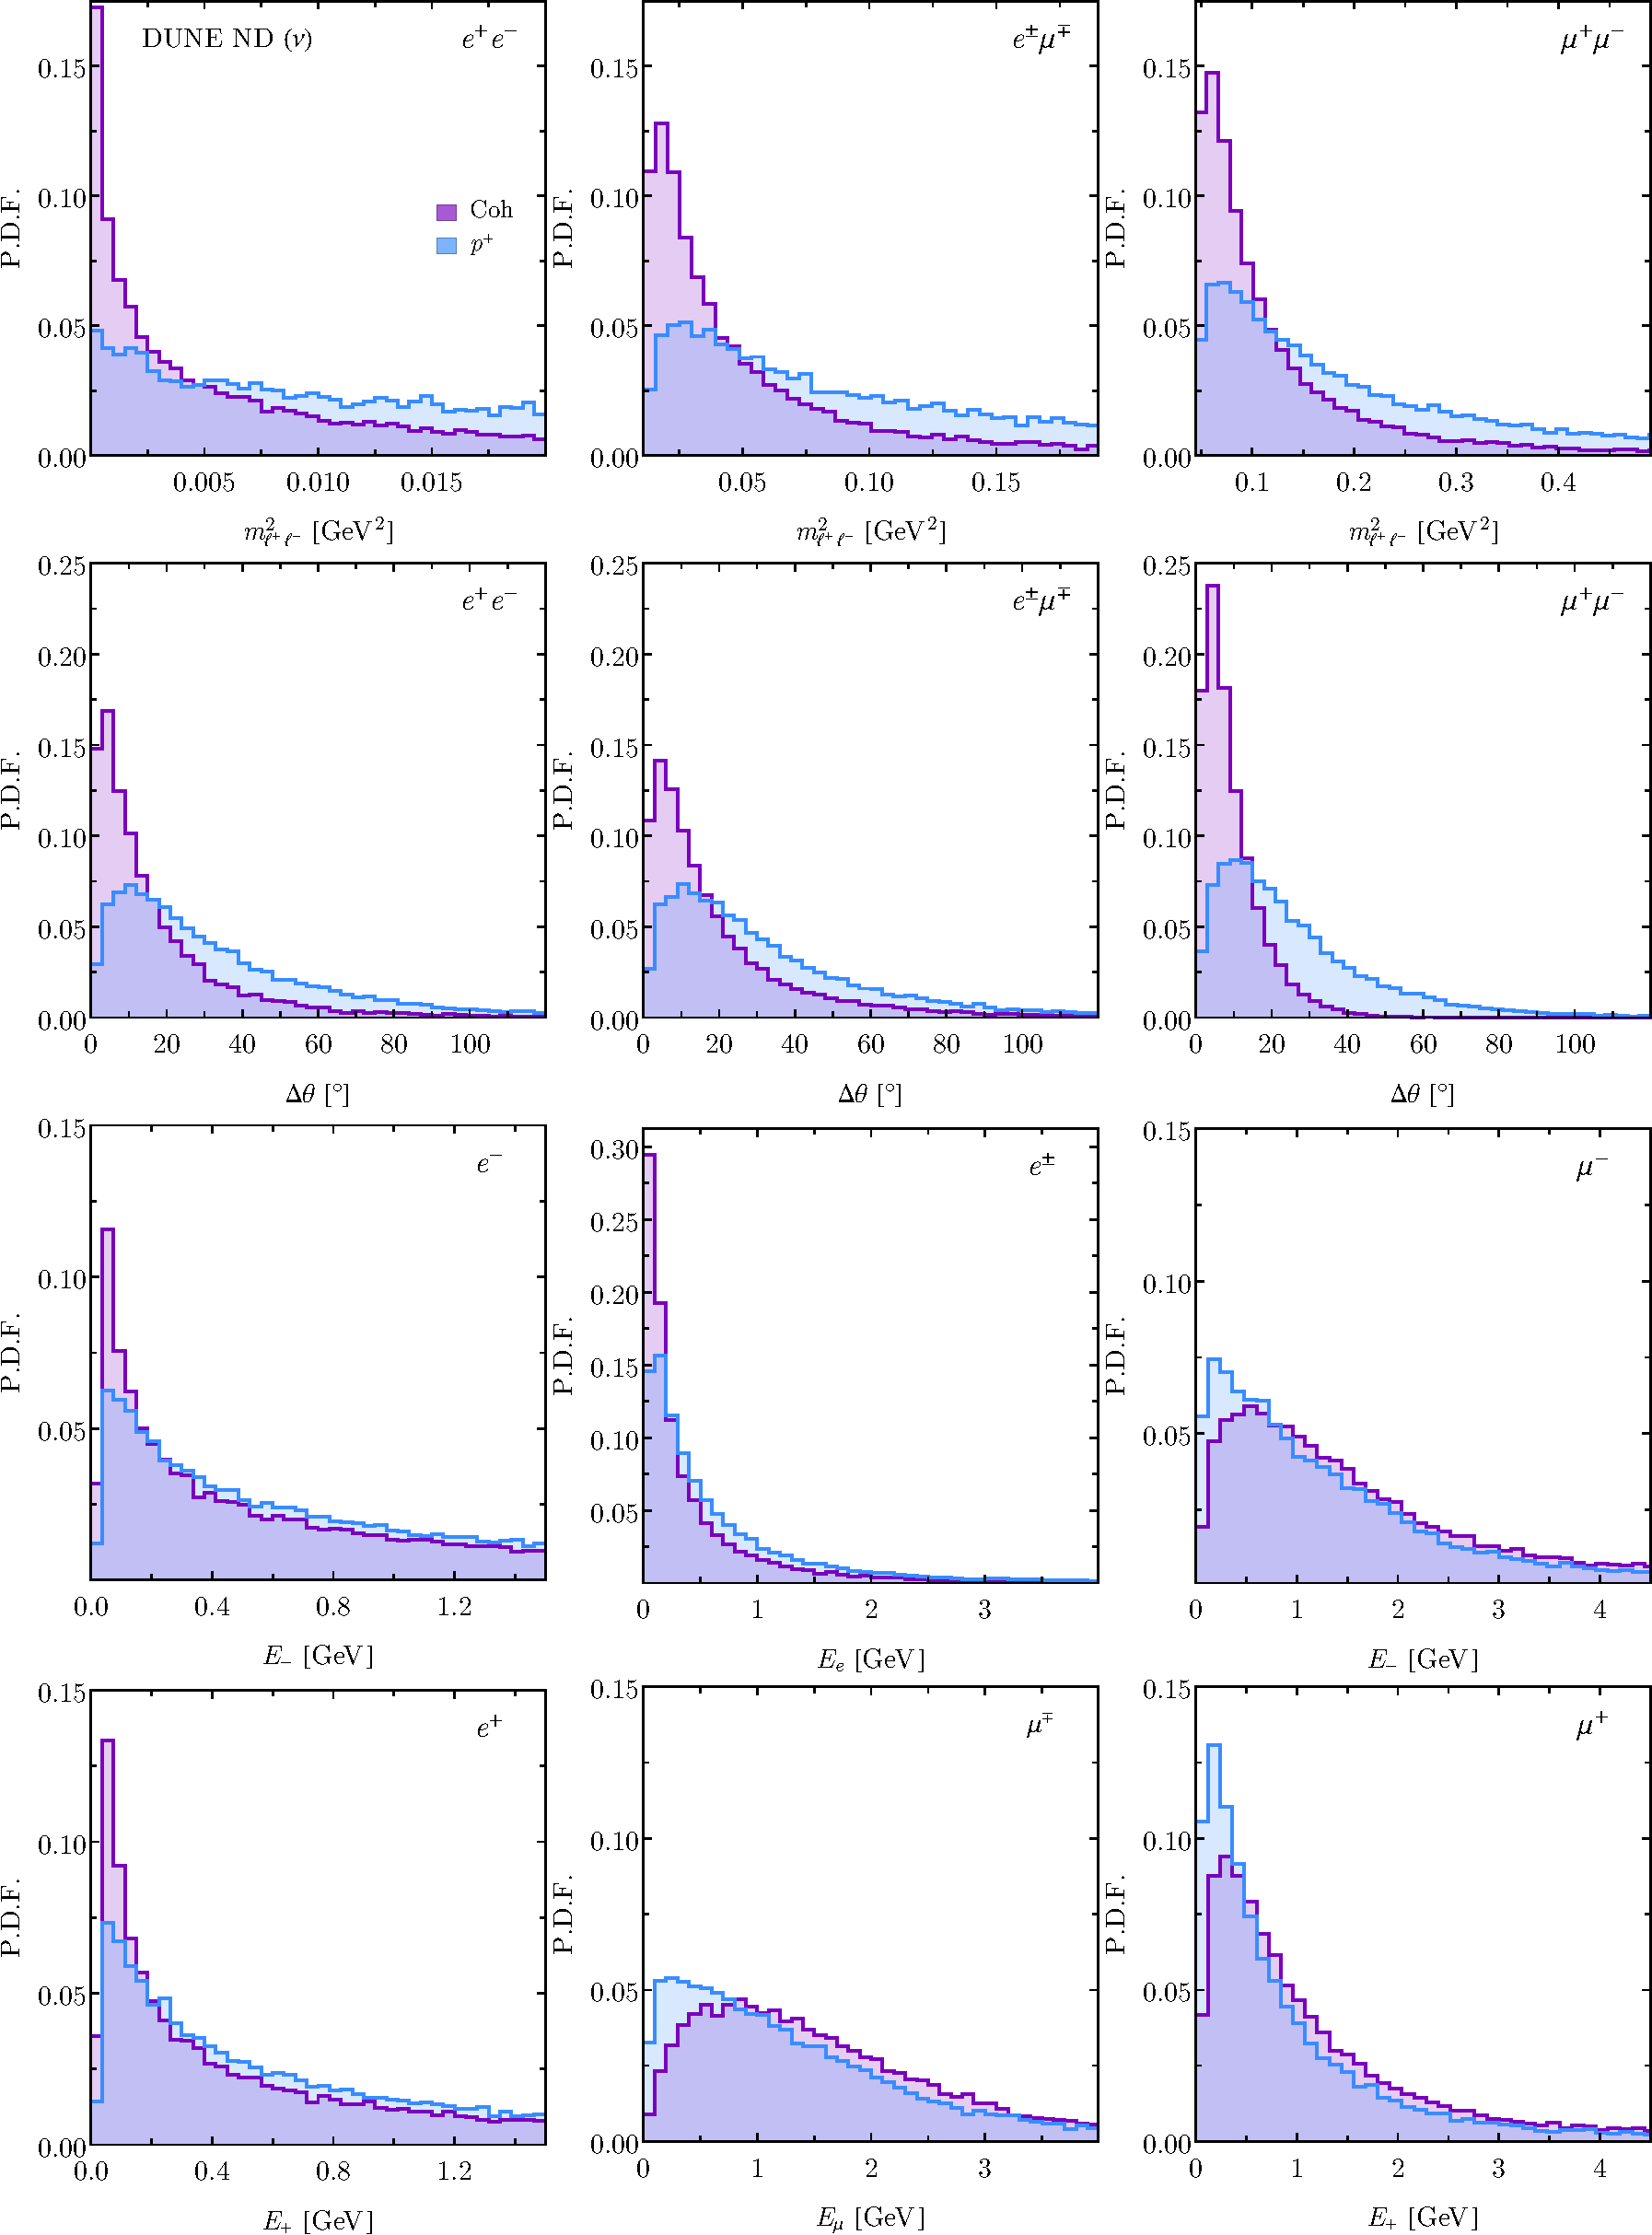
\includegraphics[width=\textwidth]{figs/DUNE_nu_3horn_mll_theta_E.pdf}
\caption{Flux convolved neutrino trident production distributions for DUNE ND in neutrino mode. In purple we show the coherent contribution in $^{40}$Ar and in blue the diffractive contribution from protons as targets only (including Pauli blocking). The coherent and diffractive distributions are normalized independently. The relative importance of each contribution as a function of $E_\nu$
can be seen in Fig.~\ref{fig:RatioCDvsT}.
%
\label{fig:DUNE_ND_dist}}
\end{figure}
%
\begin{figure}[H]
\centering
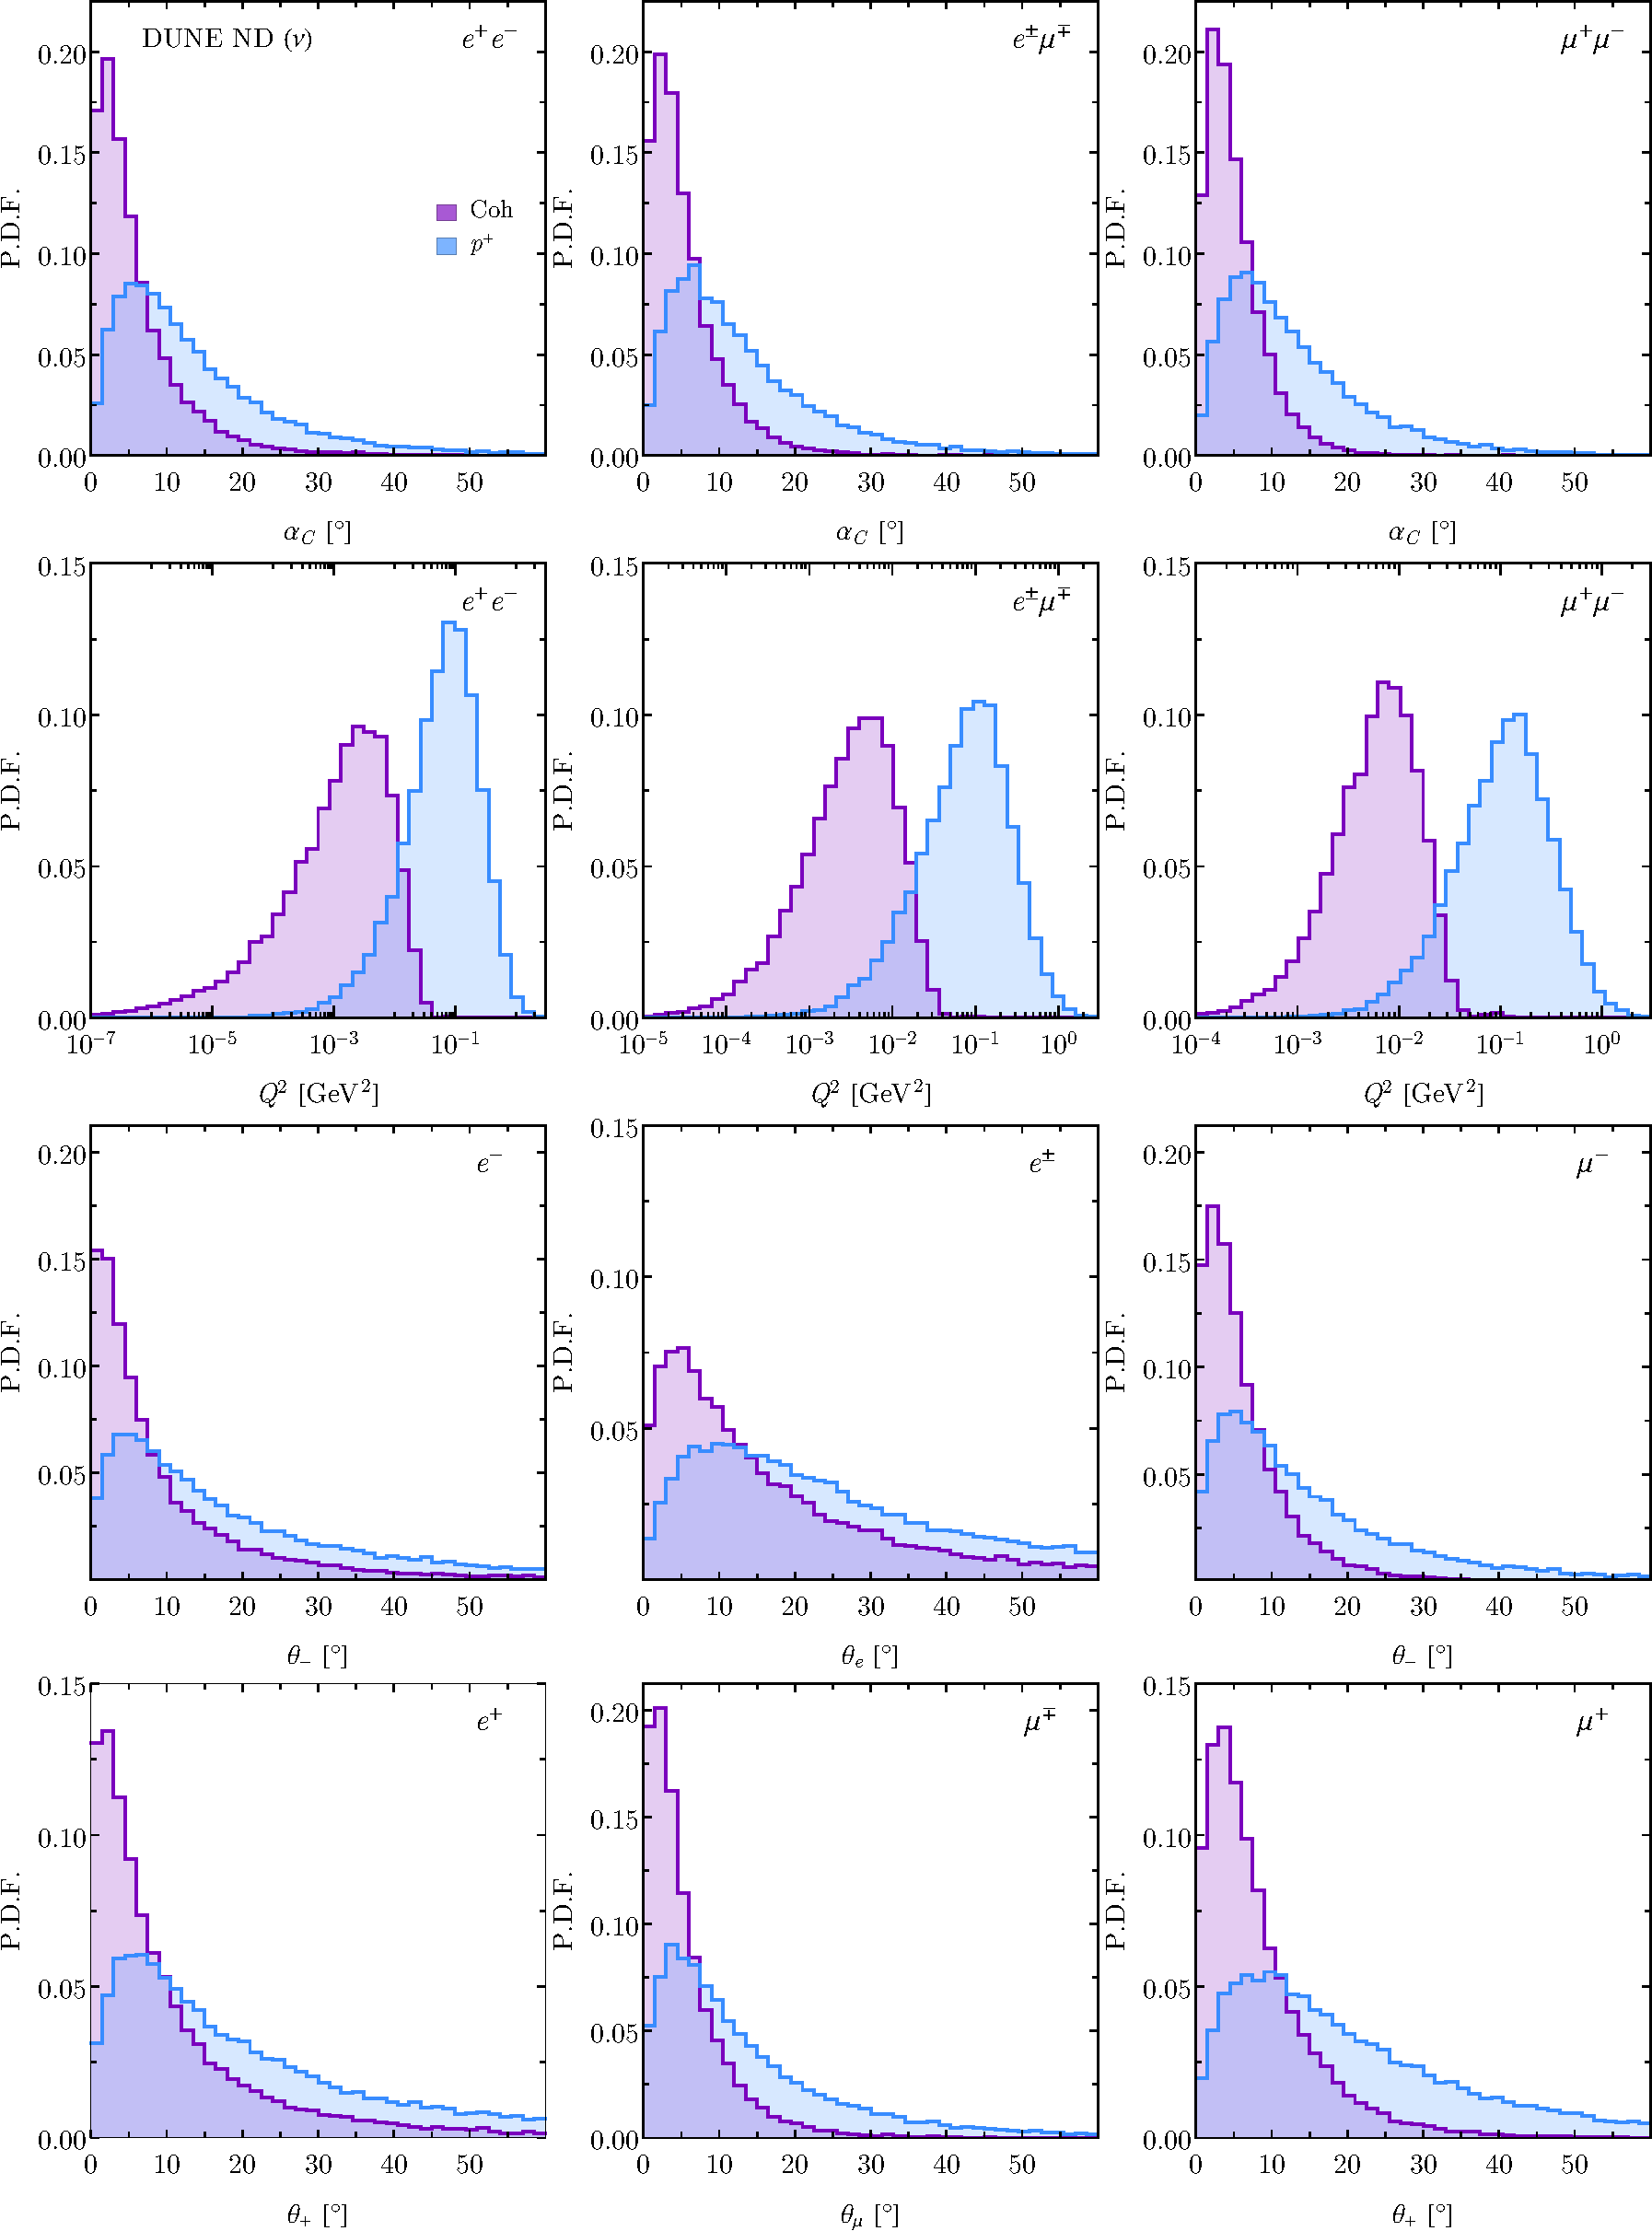
\includegraphics[width=0.92\textwidth]{figs/DUNE_nu_3horn_aC_Q2_thetapm.pdf}
\caption{Flux convolved neutrino trident production distributions for DUNE ND in neutrino mode in additional variables. In purple we show the coherent contribution in $^{40}$Ar and in blue the diffractive contribution from protons as targets only (including Pauli blocking). The coherent and diffractive distributions are normalized independently. \label{fig:other_dists}}
\end{figure}
%